
\section{Übersicht}

\begin{frame}
  {Übersicht}
  \begin{itemize}[<+->]
%    \item Intuitive Einführung in das Konzept der Freiheitsgrade.
    \item Wann sind Unterschiede zwischen Mittelwerten signifikant?
    \item Mittelwerte in Grundgesamtheiten und Stichproben
  \end{itemize}
\end{frame}

\begin{frame}
  {Literatur}
  \begin{itemize}
    \item \citet{GravetterWallnau2007}
    \item \citet{Bortz2010}
      \vspace{\baselineskip}
    \item oder eben gleich \citet{Fisher1935a}
  \end{itemize}
\end{frame}


\section{Wiederholungen}


\subsection{Logik von statistischen Tests}

\begin{frame}
  {Tests in Fishers Philosophie}
  \begin{enumerate}
    \item \alert{Nullhypothese} (H0) festlegen: Der theoretisch angenommene Effekt\\
      existiert \alert{nicht} (z.\,B.: Die Versuchsperson [VP] kann \alert{nicht} erkennen,\\
      ob Tee oder Milch zuerst in der Tasse war).
    \item \alert{Stichprobengröße} und \alert{Versuchsaufbau} festlegen (z.\,B.\ acht Tassen\\
      mit vier \textit{Tee zuerst}-Tassen; VP kennt das Verhältnis)
    \item \alert{\textit{sig}-Niveau} festlegen: Wie unwahrscheinlich darf das Ergebnis\\
      unter Annahme der H0 sein, damit wir die H0 zurückweisen.
    \item Experiment durchführen, Ergebnis messen.
    \item \alert{p-Wert} berechnen: Wie wahrscheinlich \alert{war} es, dieses Ergebnis\\
      oder ein extremeres Ergebnis zu erreichen, wenn die H0 die Welt korrekt beschreibt.
    \item Wenn \alert{$p\leq sig$}, dann H0 zurückweisen: Entweder der Effekt existiert\\
      (\zB die VP kann die Reihenfolge des Einschenkens erkennen)\\
      \alert{oder ein seltenes Ereignis ist eingetreten}.
  \end{enumerate}
\end{frame}

\begin{frame}
  {Einschränkungen und Probleme bei der Interpretation}
  \begin{itemize}
    \item Voraussetzung: \alert{echte Zufallsstichprobe}
    \item Ergebnis: \alert{kein Beweis}
    \item keine Auskunft darüber, wie "`wahrscheinlich"' der Effekt ist
    \item keine Auskunft darüber, wie stark wir von der Existenz des Effekts\\
      überzeugt sein sollten (= \textit{inverse probability})
    \item jede H0-Zurückweisung: nur ein kleinteiliger Hinweis auf einen Effekt
    \item \alert{substantielle} theoretische Hypothese oft und hart testen!
      \vspace{\baselineskip}
    \item \alert{Sensitivity}: keine Auskunft über die \alert{Stärke} des Effekts
      \begin{itemize}
        \item große Stichprobe $\rightarrow$ hohe Sensitivität
        \item kleine Strichprobe $\rightarrow$ niedrige Sensitivität
        \item je sensitiver desto leichter werden schwache Effekte signifikant
        \item Abhilfe bei Neyman-Pearson: \alert{Power} (Teststärke) vor dem Experiment
        \item quasi-kompatibel zu Fisher: \alert{Effektstärke} nach dem Experiment
      \end{itemize}
  \end{itemize}
\end{frame}

\begin{frame}
  {Und beim Konfidenzintervall?}
  Am Beispiel des 95\%-Konfidenzintervalls (KI)
  \begin{itemize}
    \item \rot{Falsch}: Wir können zu 95\% sicher sein, dass der wahre Wert im KI liegt.
    \item \rot{Falsch}: Der wahre Wert liegt mit 95\% Wahrscheinlichkeit im KI.
      \vspace{\baselineskip}
    \item Warum? \alert{Wenn der wahre Wert nicht im geschätzten KI liegt,\\
      ist die Wahrscheinlichkeit 1, dass er nicht im KI liegt.}
    \item Fakten haben die Wahrscheinlichkeit 1.
      \vspace{\baselineskip}
    \item Richtig: Entweder liegt der wahre Wert im KI\\
      \alert{oder ein seltenes Ereignis ist eingetreten}
    \item "`selten"' heißt: nur in 5 von 100 Fällen (im Grenzwert)
  \end{itemize}
\end{frame}


\begin{frame}
  {Exakter vs.\ asymptotischer Test}
  \begin{itemize}
    \item \alert{exakter} Test: 
      \begin{itemize}
        \item Die Wahrscheinlichkeitverteilung ist bekannt und wird direkt\\
          zugrunde gelegt (= Berechnung der exakten Wahrhscheinlichkeit).
        \item Fisher-Test, Binomialtest
        \item hohe Sensitivität
        \item geeignet für kleine Stichproben
        \item oft rechenintensiv
      \end{itemize}
    \vspace{\baselineskip}
    \item \alert{approximativer} oder \alert{asymptotischer} Test: 
      \begin{itemize}
        \item Die Wahrscheinlichkeitsverteilung ist nicht bekannt\\
          (oder kann mathematisch nicht effizient zugrundegelegt werden)\\
          und es wird ein Differenzwert berechnet, der asymptotisch\\
          eine bekannte Verteilung hat.
        \item $\chi^2$-Test, t-Test, ANOVA
        \item oft wird Normalverteilung approximiert
        \item wegen asymptotischer Natur weniger sensitiv (= größere Stichprobe)
      \end{itemize}
  \end{itemize}
\end{frame}

\begin{frame}
  {Parametrische und nichtparametrische Tests}
  \begin{itemize}
    \item \alert{parametrischer Test}:
      \begin{itemize}
        \item Messung eines Parameters\slash mehrerer Parameter der Grundgesamtheit
        \item (Parameter entsprechen in der Messung einer Variable)
        \item zum Beispiel Mittelwert oder Varianz
        \item Voraussetzung: \alert{bekannte Wahrscheinlichkeitsverteilung der Variable}
        \item \zB t-Test (mittel), ANOVA (Varianz)
      \end{itemize}
    \vspace{\baselineskip}
    \item \alert{nichtparametrischer Test}:
      \begin{itemize}
        \item keine direkte Messung eines zufallsverteilten Parameters
        \item zum Beispiel Ränge oder Zähldaten
        \item keine Verteilungsannahmen (auch: \textit{verteilungsfreier Test})
        \item \zB $\chi^2$, Binomialtest, H-Test, U-Test
      \end{itemize}
  \end{itemize}
\end{frame}


%\subsection{Freiheitsgrade}
%
%\begin{frame}
%  {Freiheitsgrade "`intuitiv"'}
%  \begin{itemize}[<+->]
%    \item Beispiel: Schätzung eines Parameters (\zB Mittel)\\
%      auf Basis von 1000 gemessenen Werten
%    \item Wenn 999 Werte bekannt sind,\\
%      steht abhängig vom Mittel der 1000ste Wert fest.
%    \item Für jedes Mittel $\mu$ einer Stichprobe mit $n$ Messungen\\
%      sind nur $n-1$ frei wählbar.
%  \end{itemize}
%\end{frame}
%
%\begin{frame}
%  {(Unintuitive) Erweiterung(en)}
%  \begin{itemize}[<+->]
%    \item generell: \alert{$df=n-|E|$}\\
%      wobei $E$ die zu schätzenden Parameter und $|E|$ ihre Anzahl ist.
%    \item Warum bei \alert{$\chi^2$} dann \alert{$df=(Zeilenzahl-1)\cdot(Spaltenzahl-1)$}?
%    \item Bsp.: Tabelle mit $2\times3$ Feldern, also $df=(2-1)(3-1)=1\cdot2=2$\ldots
%    \item Bei bekannten Randsummen sind aber tatsächlich nur 2 Felder frei wählbar!
%  \end{itemize}
%  \begin{center}
%    \visible<4->{
%      \begin{tabular}[h!]{|c|c|c|c}
%	\cline{2-3}
%	\multicolumn{1}{c|}{}& X1 & X2 \\
%	\cline{1-3}
%	Y1 & $\oplus$ & & ZS1 \\
%	\cline{1-3}
%	Y2 & $\oplus$ & & ZS2 \\
%	\cline{1-3}
%	Y3 & & & ZS3 \\
%	\cline{1-3}
%	\multicolumn{1}{c}{}& \multicolumn{1}{c}{SQ1} & \multicolumn{1}{c}{SQ2} & \\
%      \end{tabular}
%    }
%  \end{center}
%\end{frame}


\section[t-Test]{t-Test}

\subsection{t-Test mit einer Stichprobe}

\begin{frame}
  {Fragestellung beim z-Test und beim Einstichproben-t-Test}
  \begin{itemize}[<+->]
    \item Mittel $\mu$ über $X$ in der Grundgesamtheit bekannt\\
      (\zB mittlere Satzlänge im Korpus).
    \item Stichprobe (\zB der Grundriss von PE) zeigt gemessenes Mittel $\bar{x}$.
    \item Ist die Abweichung signifikant?
    \item \alert{H0: $\bar{x}=\mu$}
  \end{itemize}
\end{frame}

\begin{frame}
  {z-Test}
    Wäre die \alert{Varianz der GG} als $s^2(X)$ bekannt:\\
    \vspace{0.5cm}
    \begin{itemize}[<+->]
      \item SF(X) bei Stichprobengröße $n$ ausrechnen, und\ldots
      \item mit \alert{$z=\frac{\bar{x}-\mu}{SF(X)}$} einen Signifikanztest über Normalverteilung rechnen
        \vspace{\baselineskip}
      \item Problem aber leider: $SF(X)=\frac{s(X)}{\sqrt{n}}$
      \item und $s^2(X)$ meist nicht bekannt!
    \end{itemize}
    \vspace{\baselineskip}
    Aufgabe: Mit Ihrer Stichprobe aus NaB und $\mu=6.8$ sowie $s^2(X)=10.8$ z-Test rechnen. (Bzw.\ erstmal die nötigen Werte ausrechnen. Wir besprechen dann die Interpretation als Test.)
\end{frame}

\begin{frame}
  {Annahme beim t-Test mit einer Stichprobe}
  \begin{itemize}[<+->]
    \item Wir kennen $\mu$ oder haben eine Hypothese (\zB $\mu=0.5$).
    \item Wir haben eine Stichprobe $x$ mit $n$ und bekannten $\bar{x}$ und $s^2(x)$.
        \vspace{\baselineskip}
    \item anders als bei z-Test: \alert{Wir schätzen $SF(X)\approx SF(x)$!}
  \end{itemize}
\end{frame}

\begin{frame}
  {t-Formel}
  \begin{center}
    \alert{$t=\frac{\bar{x}-\mu}{SF(x)}$}
  \end{center}
  \vspace{1cm}
  \visible<2->{
    \begin{center}
      Bitte rechnen für Satzlängen (in Wörtern):\\
      $\mu=7.3$\\
      $x=[6, 3, 12, 16, 8, 15, 9, 9, 2, 11]$
    \end{center}
  }
\end{frame}

\begin{frame}
  {Lösung}
  \begin{enumerate}[<+->]
    \item $\bar{x}=9.1$
    \item $s^2(x)=21.43$
    \item $s(x)=4.63$
    \item $SF(x)=\frac{4.63}{\sqrt{10}}=1.464$
    \item $t=\frac{9.1-7.3}{1.464}=1.229$
  \end{enumerate}
  \pause
  \begin{center}
    \alert{Und was sagt uns $t=1.229$?}
  \end{center}
\end{frame}

\begin{frame}
  {t-Verteilung}
    Während die z-Werte normalverteilt sind,\\
    flacht die Verteilung der t-Werte durch die Schätzung\\
    je nach $df$ verglichen mit der Normalverteilung ab.\\
    \vspace{-0.5cm}
    \begin{center}
      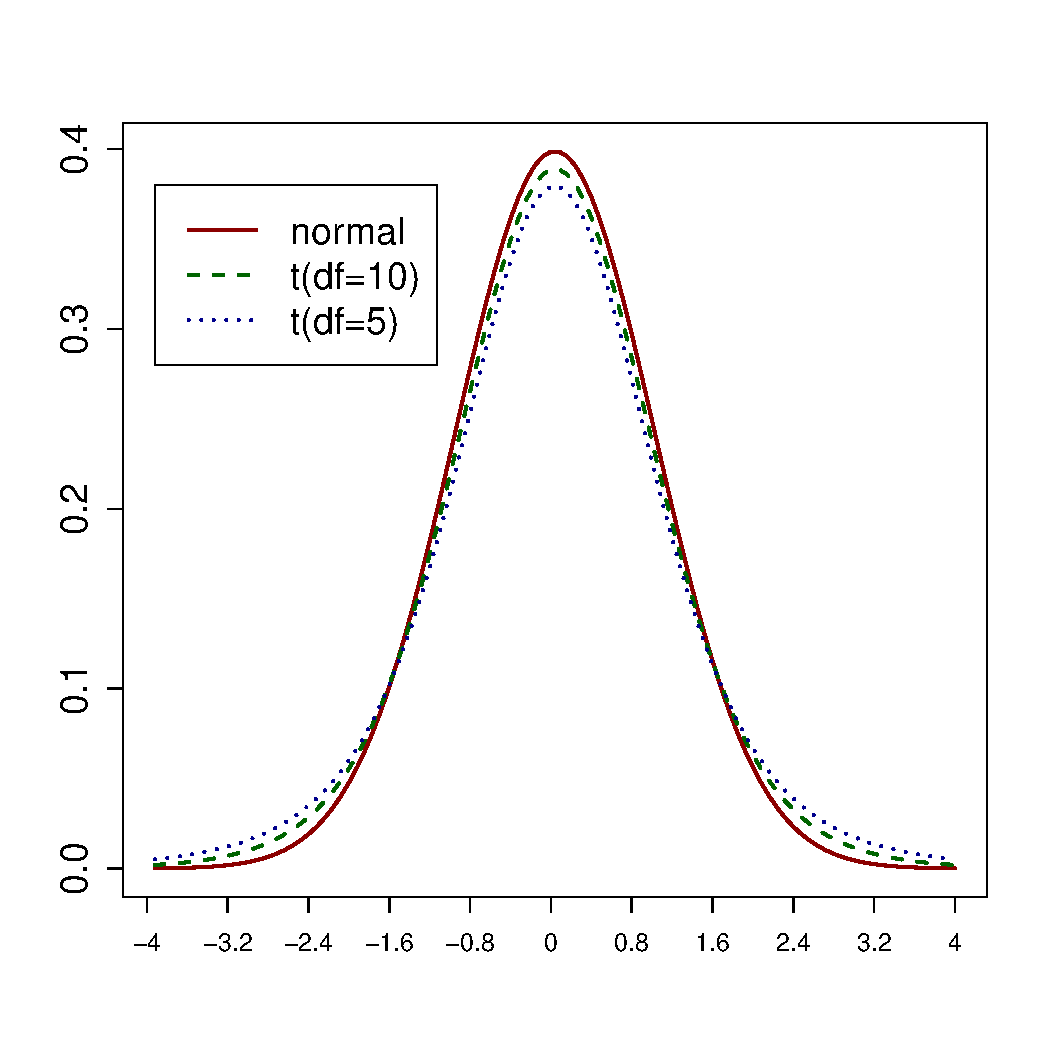
\includegraphics[width=0.5\textwidth]{tnorm}
    \end{center}
\end{frame}

% pdf("tnorm.pdf")
% plot(dnorm(x=seq(-4,4,length=100)), type="l", lwd=2, col="darkred", xlab="", ylab="", cex.axis=1.5, xaxt="n")
% axis(1,seq(0,100,length=11), labels=round(seq(-4,4,length=11), 2), cex=1.5)
% lines(dt(x=seq(-4,4,length=100), df=10), type="l", lwd=2, col="darkgreen", lty=2)
% lines(dt(x=seq(-4,4,length=100), df=5), type="l", lwd=2, col="darkblue", lty=3)
% legend(1,0.38,legend=c("normal","t(df=10)","t(df=5)"), col=c("darkred", "darkgreen","darkblue"), lty=c(1,2,3), lwd=2, cex=1.5)
% dev.off()

\begin{frame}
  {$df$ und Signifikanz}
  \begin{itemize}[<+->]
    \item \alert{$df=n-1$} ($\bar{x}$ muss für $s^s(x)$ bekannt sein)
    \item Welche t-Werte machen $1-\alpha$ der Werte aus?
    \item \texttt{> qt(c(0+0.05/2, 1-0.05/2), df=9)\\
      $\Rightarrow 2.262157 .. -2.262157$}
    \item Der errechnete t-Wert ist nicht signifikant.
    \item H0: $\mu=\bar{x}$ nicht zurückgewiesen.
  \end{itemize}
\end{frame}

\begin{frame}
  {Effektstärke}
  \begin{itemize}[<+->]
    \item Signifikanz $\neq$ starker Effekt
    \item Effektstärke beim t-Test für Stichprobe $x$:
  \end{itemize}
  \pause
  \begin{center}
    \alert{Cohens $d=\frac{\bar{x}-\mu}{s(x)}$}
  \end{center}
  \pause
  \begin{itemize}
    \item Herleitung\slash Erklärung: Gravetter \& Wallnau, Kap.\ 9
  \end{itemize}
\end{frame}

\begin{frame}
  {Erklärung der Varianz}
  \begin{itemize}
    \item ähnlich der Effektstärke: \\
      \alert{Welcher Anteil der Varianz in den Daten\\
      wird durch die Unabhängige erklärt?}
  \end{itemize}
  \pause
  \begin{center}
    \alert{Cohens $r^2=\frac{t^2}{t^2+df}$}
  \end{center}
  \pause
  \begin{itemize}
    \item Herleitung\slash Erklärung: Gravetter \& Wallnau, Kap.\ 9
  \end{itemize}
\end{frame}

\subsection{t-Test mit zwei Stichproben}

\begin{frame}
  {Zwei-Stichproben t-Test}
  \begin{itemize}[<+->]
    \item \alert{zwei Grundgesamtheiten} (\zB dt.\ Sätze im 19.\ und im 20.\ Jh.)
    \item dazu: \alert{zwei Stichproben} (je eine) mit einem \alert{Mittelwert} (\zB Länge)
    \item Interesse: anhand der \alert{zwei Stichproben} zeigen,\\
      dass sie (sehr wahrscheinlich) \alert{aus zwei Grundgesamtheiten} kommen
    \item \alert{H0: $\mu_1-\mu_0=0$}
    \item hier also: eine unabhängige Variable (Jahrhundert)\\
      und eine abhängige Variable (Satzlänge), gemessen als Mittel
  \end{itemize}
\end{frame}

\begin{frame}
  {Genereller Ansatz}
  Allgemein funktioniert der t-Test \alert{immer} so:
  \begin{center}
    \alert{$t=\frac{Stichprobenwert-Grundgesamtheitswert}{Standardfehler}$}
  \end{center}
  \pause
  Jetzt geht man per Hypothese von zwei GG und zwei Stichproben aus, also:
  \pause
  \begin{center}
    \alert{$t=\frac{(\bar{x_1}-\bar{x_2})-(\mu_1-\mu_2)}{SF(x_1-x_2)}$}
  \end{center}
  \pause
  \begin{itemize}[<+->]
    \item Wir testen also auf die \alert{Differenz der Unterschiede}.
    \item Per H0 wird gesetzt: \alert{$\mu_1-\mu_2=0$}
  \end{itemize} 
\end{frame}

\begin{frame}
  {Schätzung des Standardfehlers}
  Für \alert{gleichgroße Stichproben}:
  \begin{center}
    \alert{$SF(\bar{x_1}-\bar{x_2})=\sqrt{\frac{s^2(x_1)}{n_1}+\frac{s^2(x_2)}{n_2}}$}
  \end{center}
  \pause
  \begin{itemize}[<+->]
    \item Problem: Beitrag zum SF von beiden Stichproben gleich.
    \item Besser: \alert{zusammengefasste Varianz}, und daraus dann SF.
  \end{itemize}
  \pause
  \begin{center}
    \alert{$s^2_p(x_1,x_2)=\frac{(\sum\limits_{i=1}^{n}(x_{1,i}-\bar{x_1})^2)+(\sum\limits_{i=1}^{n}(x_{2,i}-\bar{x_2})^2)}{(n_1-1)+(n_2-1)}=\frac{SQ(x_1)+SQ(x_2)}{(n_1-1)+(n_2-1)}$}\\
    \vspace{0.5cm}
    \pause
    \alert{$SF(x_1-x_2)=\sqrt{\frac{s^2_p(x_1,x_2)}{n_1}+\frac{s^2_p(x_1,x_2)}{n_2}}$}
  \end{center}
  \pause
  \footnotesize
  Mehr: Gravetter \& Wallnau, Kap.\ 10
\end{frame}

\begin{frame}
  {Illustration der zusammengefassten Varianz}
  \begin{center}
    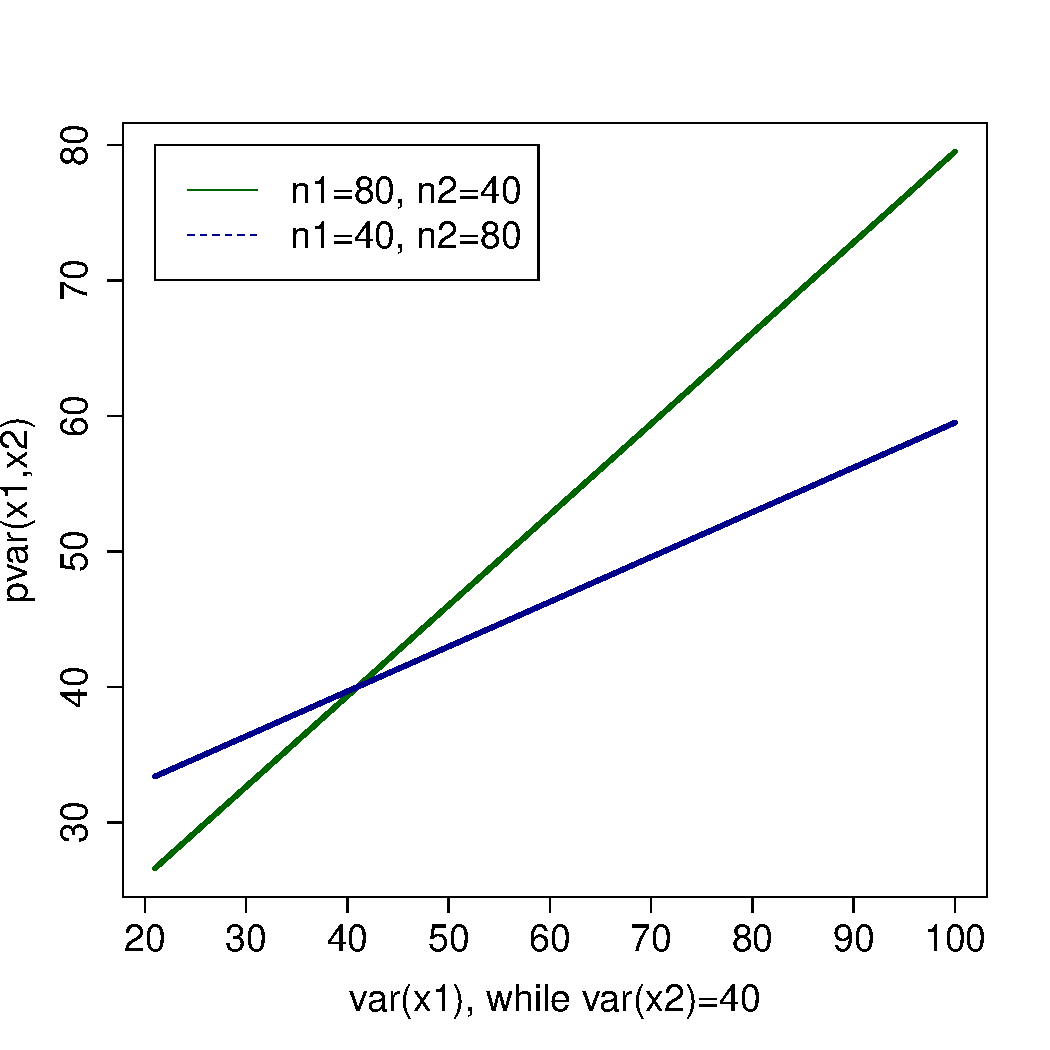
\includegraphics[width=0.5\textwidth]{pvar}
  \end{center}
\end{frame}

% pdf("pvar.pdf")
% plot(apply(vars1, 1, pv), type="l", lwd=3, cex=1.5, cex.axis=1.5, xlab="var(x1), while var(x2)=40", cex.lab=1.5, ylab="pvar(x1,x2)", col="darkgreen", xaxt="n")
% axis(1, at=seq(0,80,by=10), labels=seq(20,100,by=10), cex.axis=1.5)
% lines(apply(vars2, 1, pv), lwd=3, col="darkblue")
% legend(1,80,legend=c("n1=80, n2=40", "n1=40, n2=80"), lty=c(1,2), col=c("darkgreen", "darkblue"), cex=1.5)
% dev.off()

\begin{frame}
  {Rechnen des Tests}
  t-Wert
  \begin{center}
    \alert{$t=$}$\frac{(\bar{x_1}-\bar{x_2})-(\mu_1-\mu_2)}{SF(x_1-x_2)}=\frac{(\bar{x_1}-\bar{x_2})-0}{SF(x_1-x_2)}=$\alert{$\frac{\bar{x_1}-\bar{x_2}}{SF(x_1-x_2)}$}
  \end{center}
  \pause
  Freiheitsgrade
  \begin{center}
    $df=df(x_1)+df(x_2)=(n_1-1)+(n_2-1)$
  \end{center}
  \pause
  Effektstärke
  \begin{center}
    $d=\frac{\bar{x_1}-\bar{x_2}}{\sqrt{s^2_p}}$
  \end{center}
  \pause
  Erklärung der Varianz
  \begin{center}
    $r^2=\frac{t^2}{t^2+df}$
  \end{center}
\end{frame}

\begin{frame}
  {Übung}
  Bitte "`von Hand in \texttt{R}"' t-Test für folgende zwei Stichproben\\
  bei $\alpha=0.05$ rechnen:\\
  \begin{center}
    $x_1=[11, 11, 8, 8, 11, 9, 8, 11, 9, 8]$\\
    $x_2=[10, 14, 14, 13, 11, 14, 10, 14, 12, 10]$
  \end{center}
  \pause
  \begin{center}
    Und überprüfen mit:\\
    \texttt{> t.test(x1, x2)}
  \end{center}
\end{frame}

\begin{frame}
  {Voraussetzungen prüfen I}
  Die \alert{GGs müssen normalerverteilt} sein:
  \begin{center}
    \texttt{shapiro.test(x)}\\
    Wenn $p\leq0.05$ wird die Nullhypothese des Shapiro-Wilk-Tests verworfen --\\
    H0: Die Werte stammen aus einer normalverteilten GG.
  \end{center}
  \pause
  Die \alert{Varianzen müssen homogen sein}:
  \begin{center}
    \texttt{var.test(x1, x2)}\\
    Auch hier: $p\leq0.05$ weist die H0 zurück (sehr informell) --\\
    H0: Die Varianzen von x1 und x2 sind homogen.
  \end{center}
\pause
\begin{center}
  \alert{Solche Tests sind umstritten, weil sie i.\,d.\,R.\ viel zu empfindlich reagieren.\\
    \citet{ZuurEa2009} empfehlen \zB grafische Methoden (bei linearen Modellen).}
\end{center}

\end{frame}


\begin{frame}
  {Voraussetzungen prüfen II}
  Wenn Voraussetzungen nicht erfüllt sind:
  \begin{itemize}[<+->]
    \item steigt das Risiko für Typ 1-Fehler
    \item nicht-parametrische Alternative nehmen
    \item Daten transformieren
    \item sich über Robustheit des Test ggü. verletzten Annahmen informieren\\
      (oft schwer zugängliche und kontroverse Spezialliteratur)
  \end{itemize}
\end{frame}
